 \documentclass[12pt] {fphw}
%Compilarea se face pdfLaTeX+MakeIndex+BibTeX
\usepackage[utf8]{inputenc}  
\usepackage[T1]{fontenc}  
\usepackage{mathpazo}  
\usepackage{graphicx}  
\usepackage{booktabs} 
\usepackage{listings}  
\usepackage{enumerate}  
\usepackage{subcaption}

\title{Tema 1}  
\author{Bodnar Florina-Alina 2A4, Ungurean Ana-Maria 2A4 } % Student name
\date{4 Noiembrie 2022} % Due date
\institute{Universitatea Alexandru Ioan-Cuza \\ Facultatea de Informatică} % Institute or school name
\class{Algorimica Grafurilor} % Course or class name
\professor{Lect dr. Olariu Florentin - Emanuel} % Professor or teacher in charge of the assignment

\begin{document}

\maketitle 

\section*{Problema 1}
\subsection*{1. (a)} 
 
Urmărind definiția componentei conexe, putem spune că numărul de componente conexe a lui G este cel puțin numărul de stații de tramvai deoarece două triplete ( ${}start_i, station_i, end_i$) și (${}start_j, station_j, end_j$) sunt adiacente dacă și numai dacă ${}station_i=station_j$ și (${}start_i, end_i$) $\cap$  (${}start_j, end_j$) $\neq$  $\emptyset$ . Astfel, vom avea cel puțin k componente conexe, k fiind numărul de stații.  Fie ${}c_i$, unde 1$\leq$i$\leq$ k, o componentă conexă a grafului G, este reprezentativă pentru ${}station_{i-1}$,
fiind formată din tripletele care sunt adiacente (tripletele au în comun  ${}station_{i-1}$ 
și îndeplinesc condiția de intersecție de mai sus). Pe lângă cele k componente conexe, putem avea ${}c_j$,componentă conexă, unde j>k,  pentru cazurile în care  ${}station_i$ se află în  mai multe componente conexe.  

\subsection*{1. (b)}

Știind că $\omega$(G)reprezintă numărul maxim de clică a lui G, iar K-clică este \ o submulțime de K noduri a grafului G, care induce un graf complet, putem spune că numărul maxim de tramvaie care se pot găsi în același timp în aceeași stație este  $\omega$(G). Răspunsul este datorat faptului că toate nodurile(tripletele) trebuie să fie adiacente (să aibă muchie între ele) pentru a fi toate în aceeași stație simultan.  

\subsection*{1. (c)}
Din subpunctul (b) $\Longrightarrow$ că numărul maxim de tramvaie care se pot găsi în același timp în aceeași stație este $\omega$(G), unde $\omega$(G) $\geq$ 1 \\ Observăm că: \\ Pentru  
$\omega$(G)=3, circuitul indus de lungime maximă este 3. \\ Pentru $\omega$(G)=4, circuitul de lungime maximă este 4, însă conține două corzi $\Longrightarrow$ lungimea maximă a unui circuit indus a lui G este 3. 
 
\begin{figure}[h] 
\begin{minipage}[c]{ .3\linewidth}
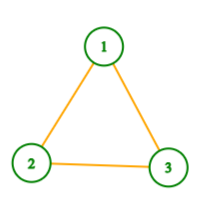
\includegraphics [height=4cm]{graph1.png}
\caption{Graf 3-clică}
\end{minipage}\hfill
\begin{minipage}[c]{.3\linewidth}
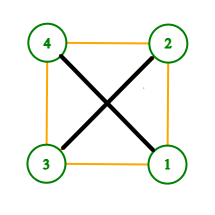
\includegraphics [height=4cm]{graph2.png}
\caption{Graf 4-clică }
\end{minipage}
\end{figure}

În graful din figura 2, circuitul de lungime 4 nu este indus, deoarece avem muchiile 1-4 și 2-3, care sunt corzi. 

\subsection*{1. (d)}
 Vom avea nevoie de o listă dublă înlănțuită, în care memorăm indicele nodului din graf și \textit{visitedNeighbors}, care inițial are doar valori de 0. Alegem să inițializăm variabila \textit{max} cu primul nod din listă. Cât timp lista e nevidă,  $\pi$[\textit{max}]=\textit{i- -}, unde \textit{i}=\textit{n} și adăugăm nodul la mulțimea S, care inițial era vidă. Apoi, eliminăm nodul \textit{max} din lista dublă înlănțuită, operație care se realizează în $\mathcal{O}$(1) (*). Parcurgem lista dublă înlănțuită și creștem cu 1 \textit{visitedNeighbors} a nodurilor care sunt vecine cu \textit{max}. La sfârșit, aleg un nod din listă a cărei valoare \textit{visitedNeighbors} este maximă. \\Astfel, operația * se realizează în $\mathcal{O}$(1) și întreg programul are timpul de execuție $\mathcal{O}$(n+m), deoarece inițializarea lui $\pi$[\textit{v}], \textit{v}$\in$ \textit{V(G)} și formarea listei dublu înlănțuite se realizează în $\mathcal{O}$(n), iar în $\mathcal{O}$(m)
are loc incrementarea \textit{visitedNeighbors} în listă și căutarea \textit{max}-ului.

\subsection*{1. (e)}
Aplicăm algoritmul de mai sus pentru subgraful indus de vecinătatea lui {$x_i$} în {$G_i$} și observăm că $\omega$(G) este reprezentată de cea mai mare valoare din vectorul  \textit{visitedNeighbors} + 1. 

\section*{Problema 2}
\subsection*{2. (a)}
Observăm că pentru orice digraf al cărui graf suport este complet, ordonarea topologică este unică și gradele interne ale nodurilor sunt distincte două câte două. Nodurile incidente cu arcul \textit{e}$\in$$A^{'}$$\setminus$$A^{"}$ vor fi interschimbate astfel încât  \textit{reverse}($\vec{G'}$, \textit{e}) este tot o orientare aciclică a lui G $\Longleftrightarrow$ gradele interioare ale nodurilor se vor interschimba. Astfel, va rezulta că ordonarea topologică a lui \textit{reverse}($\vec{G'}$, \textit{e}) este o permutare a nodurilor din $\vec{G'}$.
 
\subsection*{2. (b)}
Observăm că pentru n=1 nu putem avea un ${}K_1$, pentru care să avem 2 orientări aciclice $\vec{K'_1}$  și $\vec{K''_1}$ (pentru că \textit{E}=$\emptyset$)
$\Longrightarrow$ card( \textit{V}) $\geq$ 2. 

\begin{flushleft}
\textbf{I.} Caz de Bază: \\
Fie n=2 :

\begin{figure}[h] 
\begin{minipage}[c]{ .3\linewidth}
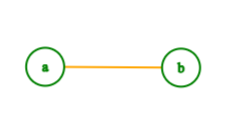
\includegraphics [height=3cm]{graph3.png}
\caption{${}K_2$}
\end{minipage}\hfill
\begin{minipage}[c]{.3\linewidth}
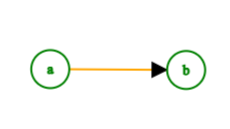
\includegraphics [height=3cm]{graph4.png}
\caption{$\vec{K'_2}$ }
\end{minipage}\hfill
\begin{minipage}[c]{ .3\linewidth}
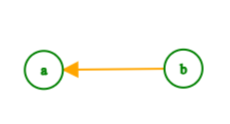
\includegraphics [height=3cm]{graph5.png}
\caption {$\vec{K''_2}$}
\end{minipage}
\end{figure}

Orientarea aciclică din figura 5 a fost determinată prin aplicarea \textit{reverse}($\vec{K'_2}$, \textit{ab}) o singură dată.  \textbf{"A"} 
\end {flushleft}

\begin{flushleft}
\textbf{II.} Presupunem P(k) adevărat, unde P(k): {$\vec{K'_k}$} poate fi transformat în  {$\vec{K''_k}$} prin aplicări repetate ale operației \textit{reverse}. 

Știm că {$K_k$} are $\frac{k(k-1)}{2}$ muchii (graf complet) $\Longrightarrow$
{$\vec{K'_k}$} și {$\vec{K''_k}$} au $\frac{k(k-1)}{2}$ muchii.  \\
$\Longrightarrow$ {$\vec{K'_k}$} și {$\vec{K''_k}$} au cel mult k-1 muchii în comun (deoarce {$\vec{K'_k}$} și {$\vec{K''_k}$}  sunt distincte și nu trebuie să aibă circuite) \\
Determinăm numărul maxim de muchii distincte
$\frac{k(k-1)}{2}$ - \textit{(k-1)} = $\frac{k(k-1)- 2k+2}{2}$ = $\frac{k^2-k-2k+2}{2}$ =$\frac{k^2-k-2(k-1)}{2}$= $\frac{k(k-1)-2(k-1)}{2}$ = $\frac{(k-1)(k-2)}{2}$ \\
$\Longrightarrow$ Putem aplica operația \textit{reverse} de maxim $\frac{(k-1)(k-2)}{2}$ ori . \textbf{"A"} 
\end {flushleft}

\begin{flushleft}
\textbf{III.}  Demonstrăm: P(k+1) adevărat, unde P(k+1): {$\vec{K'_{k+1}}$} poate fi transformat în  {$\vec{K''_{k+1}}$} prin aplicări repetate ale operației \textit{reverse}. P(k+1) : $\frac{(k)(k-1)}{2}$ ori \\

Știm că {$K_{k+1}$} are $\frac{k(k-1)}{2}$ + \textit{(k-1)} muchii  $\Longrightarrow$
{$\vec{K'_{k+1}}$} și {$\vec{K''_{k+1}}$} au $\frac{k(k-1)}{2}$ + \textit{(k-1)} muchii.  \\
$\Longrightarrow$ {$\vec{K'_k}$} și {$\vec{K''_k}$} au cel mult k muchii în comun \\
Determinăm numărul maxim de muchii distincte
$\frac{k(k-1)}{2}$ + \textit{(k-1)} - \textit{k} = $\frac{k^2-k+2k-2-2k}{2}$ =$\frac{k^2-k+2}{2}$= $\frac{k^2-3k-2+2k}{2}$ =  $\frac{k^2-3k-2}{2}$ + $\frac{2k}{2}$ = $\frac{(k-1)(k-2)}{2}$ + \textit{k} = P(k) + \textit{k} \\
$\Longrightarrow$ P(k+1) adevărat
$\Longrightarrow$ Putem aplica operația \textit{reverse} de maxim $\frac{(k-1)(k-2)}{2}$ + \textit{k} ori .  \\

$\Longrightarrow$ {$\vec{K'_n}$} poate fi transformat în {$\vec{K''_n}$} prin aplicări repetate ale operației  \textit{reverse}. 

\end {flushleft}
\subsection*{2. (c)}
Fie {$A_0$} digraful completar a lui {$\vec{G}$} $\Longleftrightarrow$ \textit{(V, A  $\bigcup$ {$A_0$) }} este o orientare aciclică a lui G cu condiția ca sumele gradelor interioare {$d_{G}^-$} (u) + {$d_{A_0}^-$} (u), unde u $\in$ \textit{V} să fie distincte două câte două (pentru a nu avea circuite) . 

\subsection*{2. (d)}
Știm că: |{$\vec{G'}$}|=|{$\vec{G''}$}| ( {$\vec{G'}$} și {$\vec{G''}$} au muchii între aceleași noduri, doar că au orientări diferite sau nu) și că suma gradelor interioare trebuie să fie aceeași. \\

\textbf{A.} De la (c), știm că orice orientare aciclică, {$\vec{G}$}, are un digraf complementar {$A_0$} astfel încât graful suport al digrafului \textit{(V, A  $\bigcup$ {$A_0$) }} este un {${K_n}$}. \\

\textbf{B.} Am demonstrat la (b) prin inducție că $\forall$  {${K_n}$}, $\exists$ {$\vec{K'_n}$} și {$\vec{K''_n}$} două orientări aciclice ale lui  {${K_n}$} și că {$\vec{K'_n}$} poate fi transformat în {$\vec{K''_n}$} prin aplicări repetate ale lui \textit{reverse}. \\

Din \textbf{A+B} $\Longrightarrow$ {$\vec{G''}$} poate fi obținut prin aplicări repetate a funcției \textit{reverse} asupra {$\vec{G'}$} 

\section*{Problema 3}
\subsection*{3}
Demonstrăm că algoritmul Dijkstra nu rulează corect în cazul în care anumite arce au cost negativ la care se adaugă o constantă pozitivă suficient de mare la costul fiecărui arc în așa fel încât toate costurile să devină pozitive, fapt susținut de contra-exemplul următor:

\begin{figure}[h] 
\begin{minipage}[c]{ .3\linewidth}
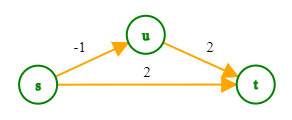
\includegraphics [height=2.5cm]{graph6.png}
\caption{G}
\end{minipage}\hfill
\begin{minipage}[c]{.3\linewidth}
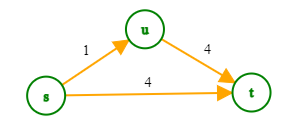
\includegraphics [height=2.5cm]{graph7.png}
\caption{G'}
\end{minipage}
\end{figure}

Să presupunem că adăugăm constanta c=2 la costul fiecărui arc din graful G, digraful rezultat este G'. \\

Aplicând algoritmul Dijkstra, obținem drumul s-u-t de cost=5, dar drumul s-t are cost minim=4. 

\section*{Problema 4}
\subsection*{4}
Algoritmul lui Dijkstra poate rezolva problema P2 pe un astfel de digraf, deoarece transformăm digraful astfel : adăugăm valoarea absolută a celui mai mic cost negativ la toate costurile nodurilor astfel încât toate costurile să fie pozitive. Neexistând circuite negative, orice muchie poate fi parcursă o singură dată pe drumul cel mai scurt. Știm că orice drum va traversa o muchie din sursă, astfel cel mai scurt drum va fi de lungimea din graful inițial + constanta pe care am adăugat-o.  

\section*{Bonus}
Pentru i=n, vecinătatea lui {$x_i$} în {$G_i$} formează chiar graful G. Dacă nodurile vecine ale lui  {$x_i$} fac parte inițial dintr-o clică, atunci vor face parte dintr-o clică de index mai mic când construim {$G_i$}. Deci, rezultă că {$N_{G_i}$}
({$x_i$}) este o clică în \textit{G}. 
 
\end{document}
